\section{Results}
\label{sec:results}

In this section we describe the results obtained from our simulations. We have 
simulated two scenarios: A square room the pedestrians exit from, and a 
corridor where pedestrians walk along the corridor from both ends, meeting in 
the middle. For each scenario we describe the parameters we have set for the 
scenario, which features we found worth measuring for this scenario, the 
results we expected, and the results we obtained. Possible remedies for any 
discrepancies between the expected and the actual results are discussed in 
section~\ref{sec:discrepancies}.

\subsection{The square room scenario}
In this scenario we simulate pedestrians leaving a square room of 10 m by 10 m 
with one exit with a width of 1 m in the middle of one of the walls. 100 
pedestrians start out spread out throughout the whole room, and head for the 
same exit. Pedestrian flow rate is measure in the door opening, and the 
density of pedestrians in a 2 m by 2 m area directly in front of the door is 
measured. We also measure the time it takes for all pedestrians to leave the room.

The parameters for this simulation are as follows:

\begin{itemize*}
    \item $A: 2,2$, $B: 0,2$, $U: 2.0$, $\lambda: 0,1$.
    \item Mean desired velocity: $1,34 m/s$, deviation $0,26 m/s$. Max 
        velocity fpedestrian $1,3$.
    \item Radius mean $0,2 m$, deviation $0,01 m$.
    \item Relaxation time: $1,0 s$.
    \item Number of pedestrians: $100$.
\end{itemize*}

% TODO: Add parameters that are varied.


\subsection{The corridor scenario}
In this scenario we simulate pedestrians walking in both directions along a 20 
m long and six metres wide corridor. The pedestrians are divided into two 
groups, starting in opposite ends of the corridor and moving towards each 
other. The targets the pedestrians move towards are set 500 metres to each 
side, to make pedestrians walk in almost a straight line instead of converging 
towards the middle of the corridor. Flow rate is measured in the middle of the 
corridor, as is density. We start out with 100 pedestrians, adding a 
continuous inflow of three pedestrians per second, to simulate people arriving 
from outside the simulated area. Both the initial placement and the inflow of 
pedestrians are distributed randomly (i.e. approximately evenly) between the 
two ends of the corridor.

We expect to see lane formations through out our simulations
and the freezing by heating effect when we start raising the mean velocity
of the agents.
In the first simulation the parameters are set after \cite{ABconstant} and
\cite{self-org}, to see if we can replecate their simulations and results.
The parameters for this simulation are as follows:

\begin{itemize*}
    \item $A: 2,2$, $B: 0,2$, $U: 2,0$, $\lambda: 0,1$.
    \item Mean desired velocity: $0,74 m/s$, deviation $0,26 m/s$. Max 
        velocity factor $1,3$.
    \item Radius mean $0,3 m$, deviation $0,01 m$.
    \item Relaxation time: $1,0 s$.
    \item Number of pedestrians: $20$ starting, adding $1/s$.
\end{itemize*}

When running the simulation we observe lane formations, and they almost clog up
in the corridor.

\begin{itemize*}
    \item $A: 2,2$, $B: 0,2$, $U: 2,0$, $\lambda: 0,1$.
    \item Mean desired velocity: $0,74 m/s$, deviation $0,26 m/s$. Max 
        velocity factor $4,0$.
    \item Radius mean $0,3 m$, deviation $0,01 m$.
    \item Relaxation time: $1,0 s$.
    \item Number of pedestrians: $20$ starting, adding $1/s$.
\end{itemize*}

When we do a simulation with the max velocity factor set to $4.0$, the clogging
that occurs in the beginning eases up, and the pedestrians relatively fast
get out of the clogging and continuous toward their target.

\begin{figure}
\centering
\subfloat[The figure show the density in corridor when the parameters are set as \cite{ABconstant} and \cite{self-org}.]{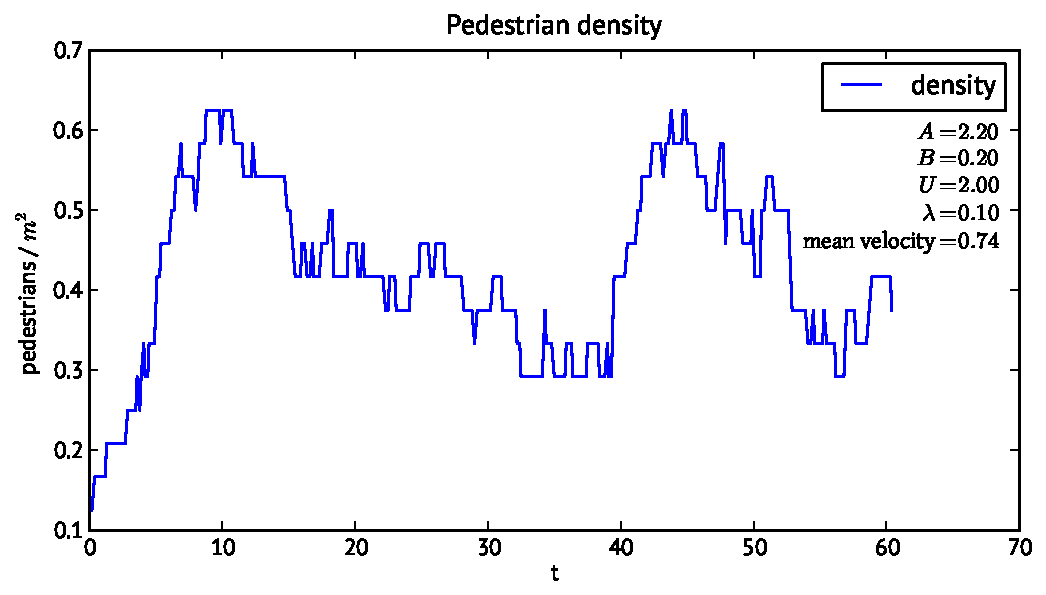
\includegraphics[scale=0.45]{Figures/dens_init_20.pdf}}
\subfloat[This figure shows the density in the corridor when the max velocity factor is set to $4.0$, and the other parameters as figure a.]{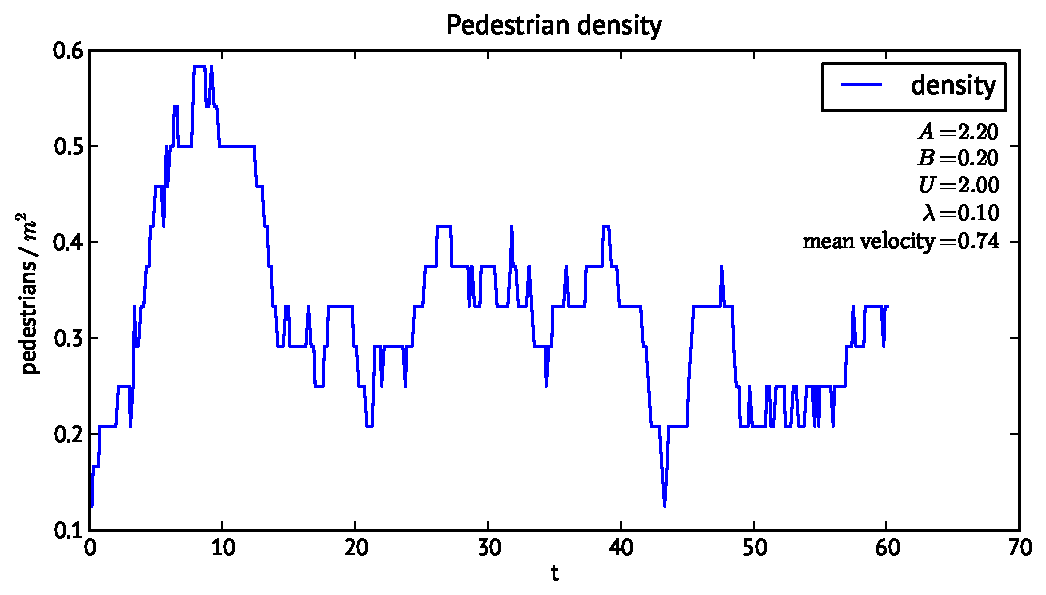
\includegraphics[scale=0.45]{Figures/dens_mvel4_20.pdf}}
\caption{These figures was made to see if the freezing by heating effect when raising the max velocity factor. As seen in the figures, the
density does not increase when the max desired velocity is increased. When raising the max desired velocity the density gets lower because
the pedestrians more easely get through the crowd.}
\label{fig:freezingbyheating}
\end{figure}
% TODO: Add parameters that are varied.
